\chapter{Appendix A.}

\begin{figure}[ht] 
	\centering
	\begin{minipage}[b]{0.5\linewidth}
		\centering
		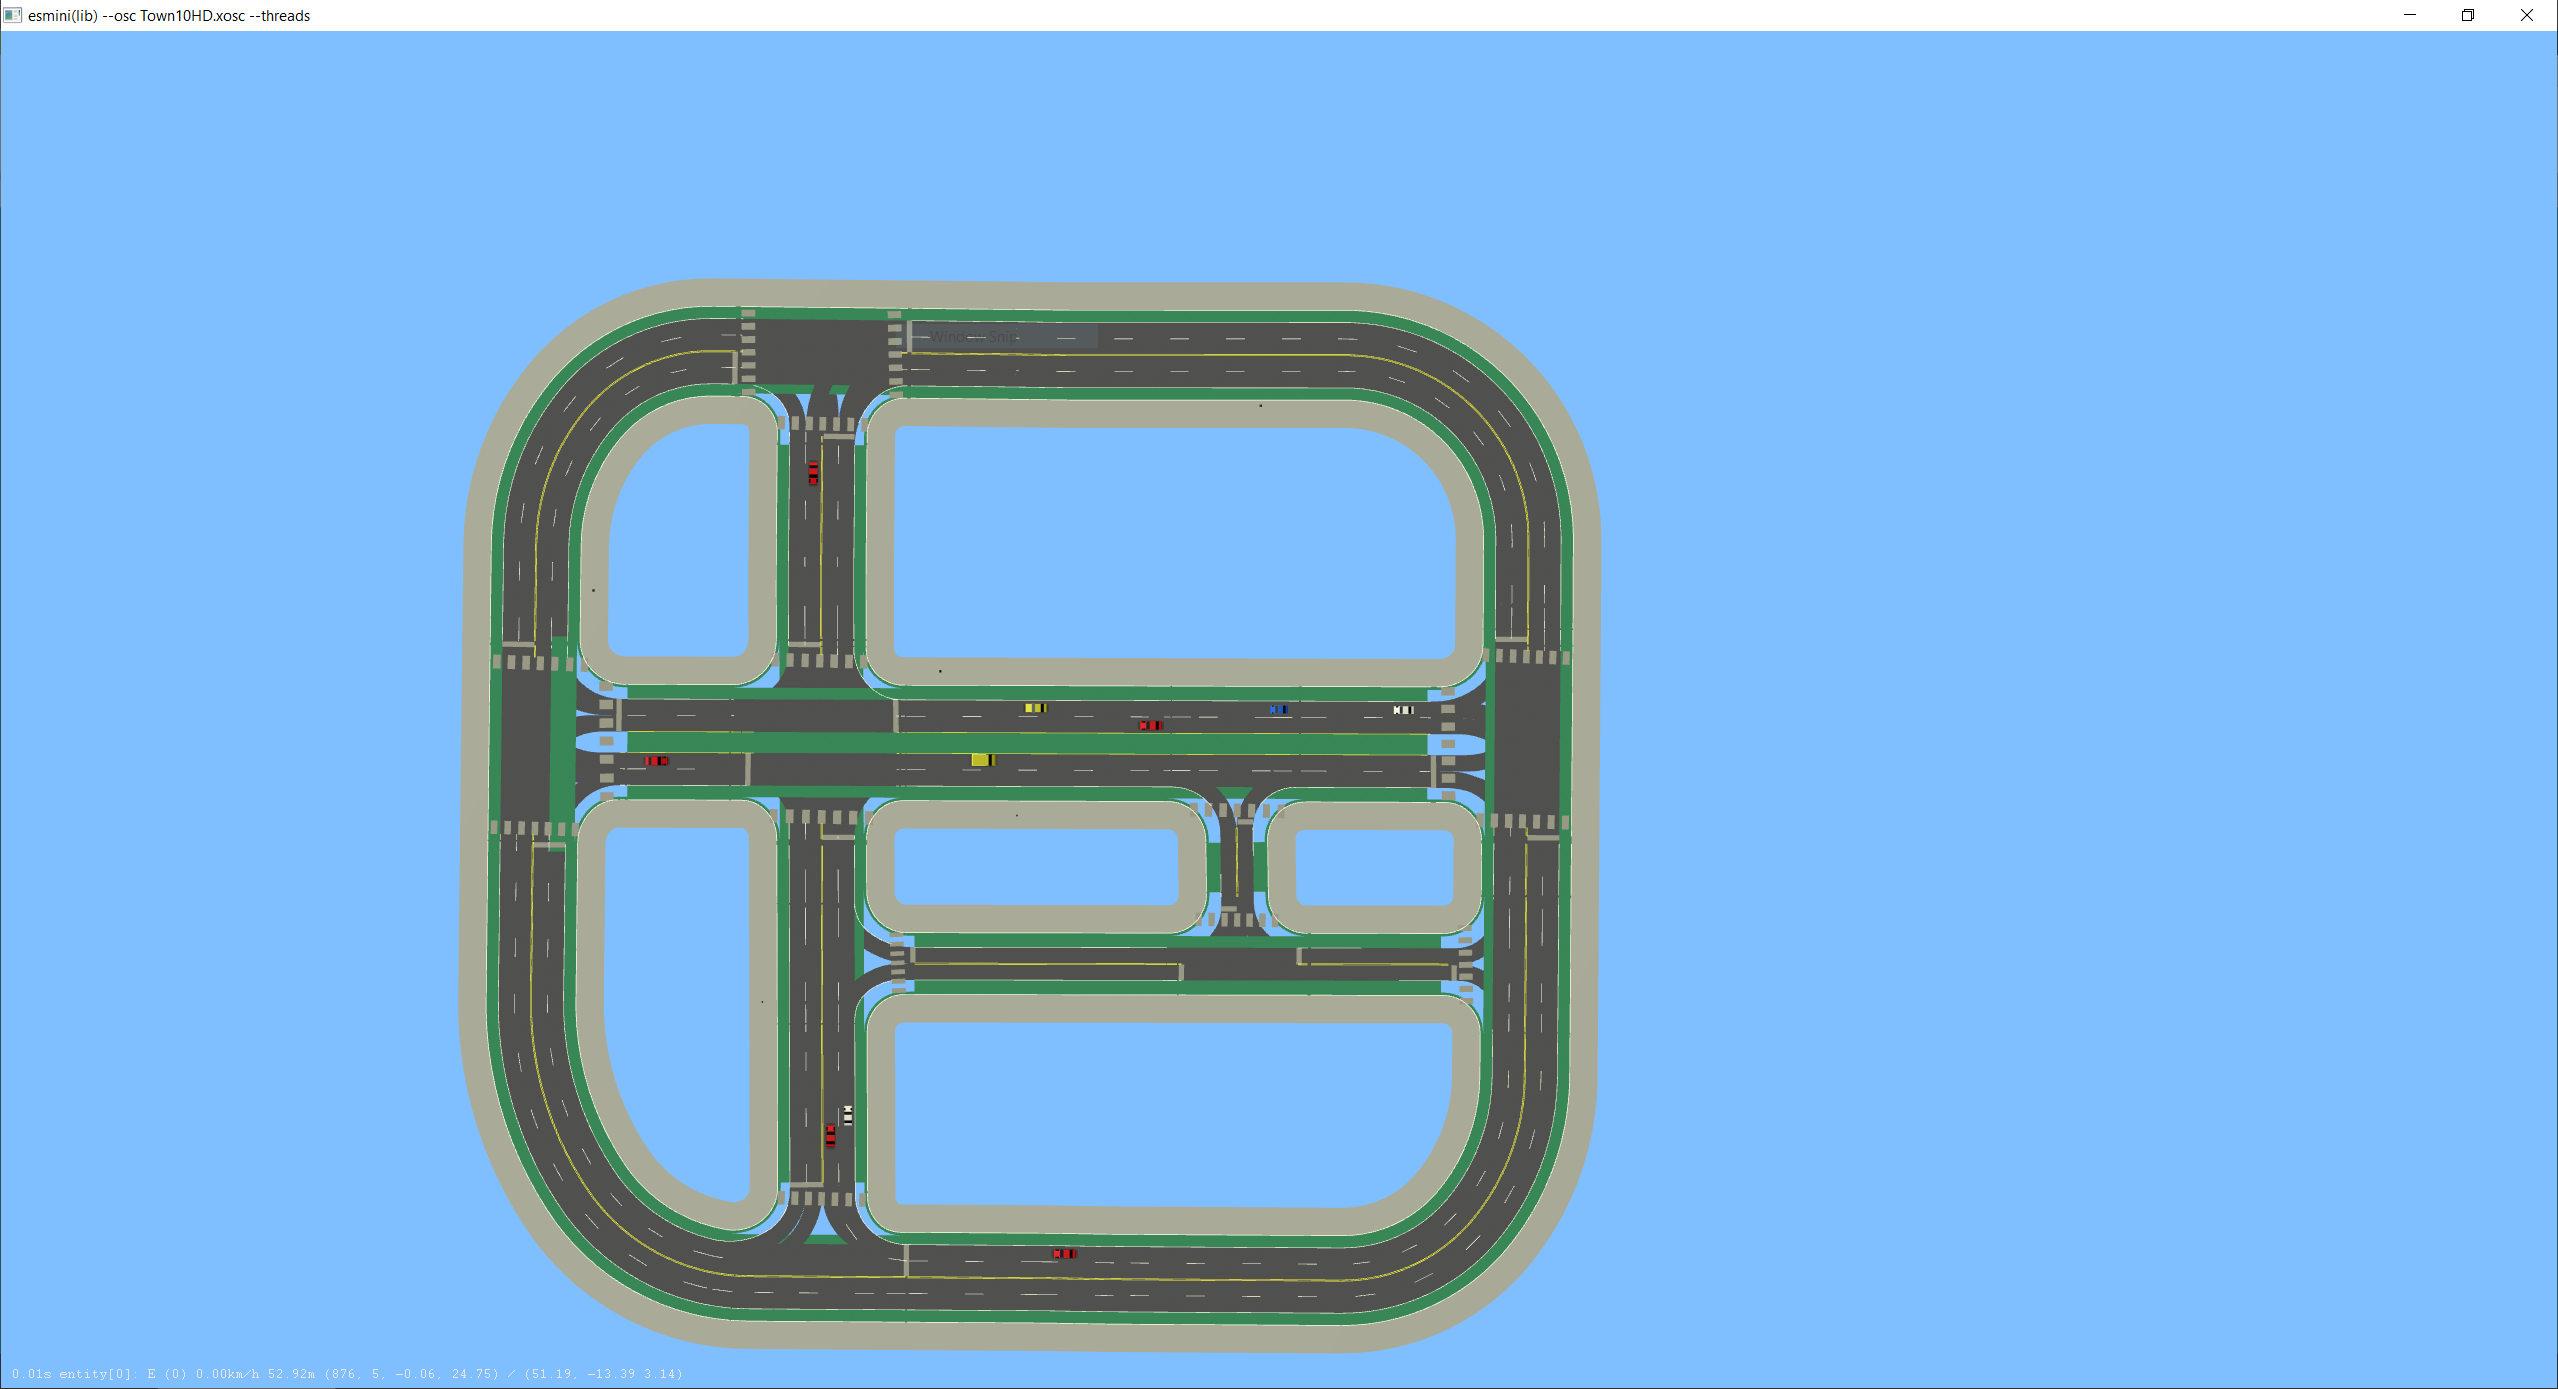
\includegraphics[width=1\linewidth]{figures/start_scenarios/scenario_1} 
		Start Scenario 1
	\end{minipage}%%
	\begin{minipage}[b]{0.5\linewidth}
		\centering
		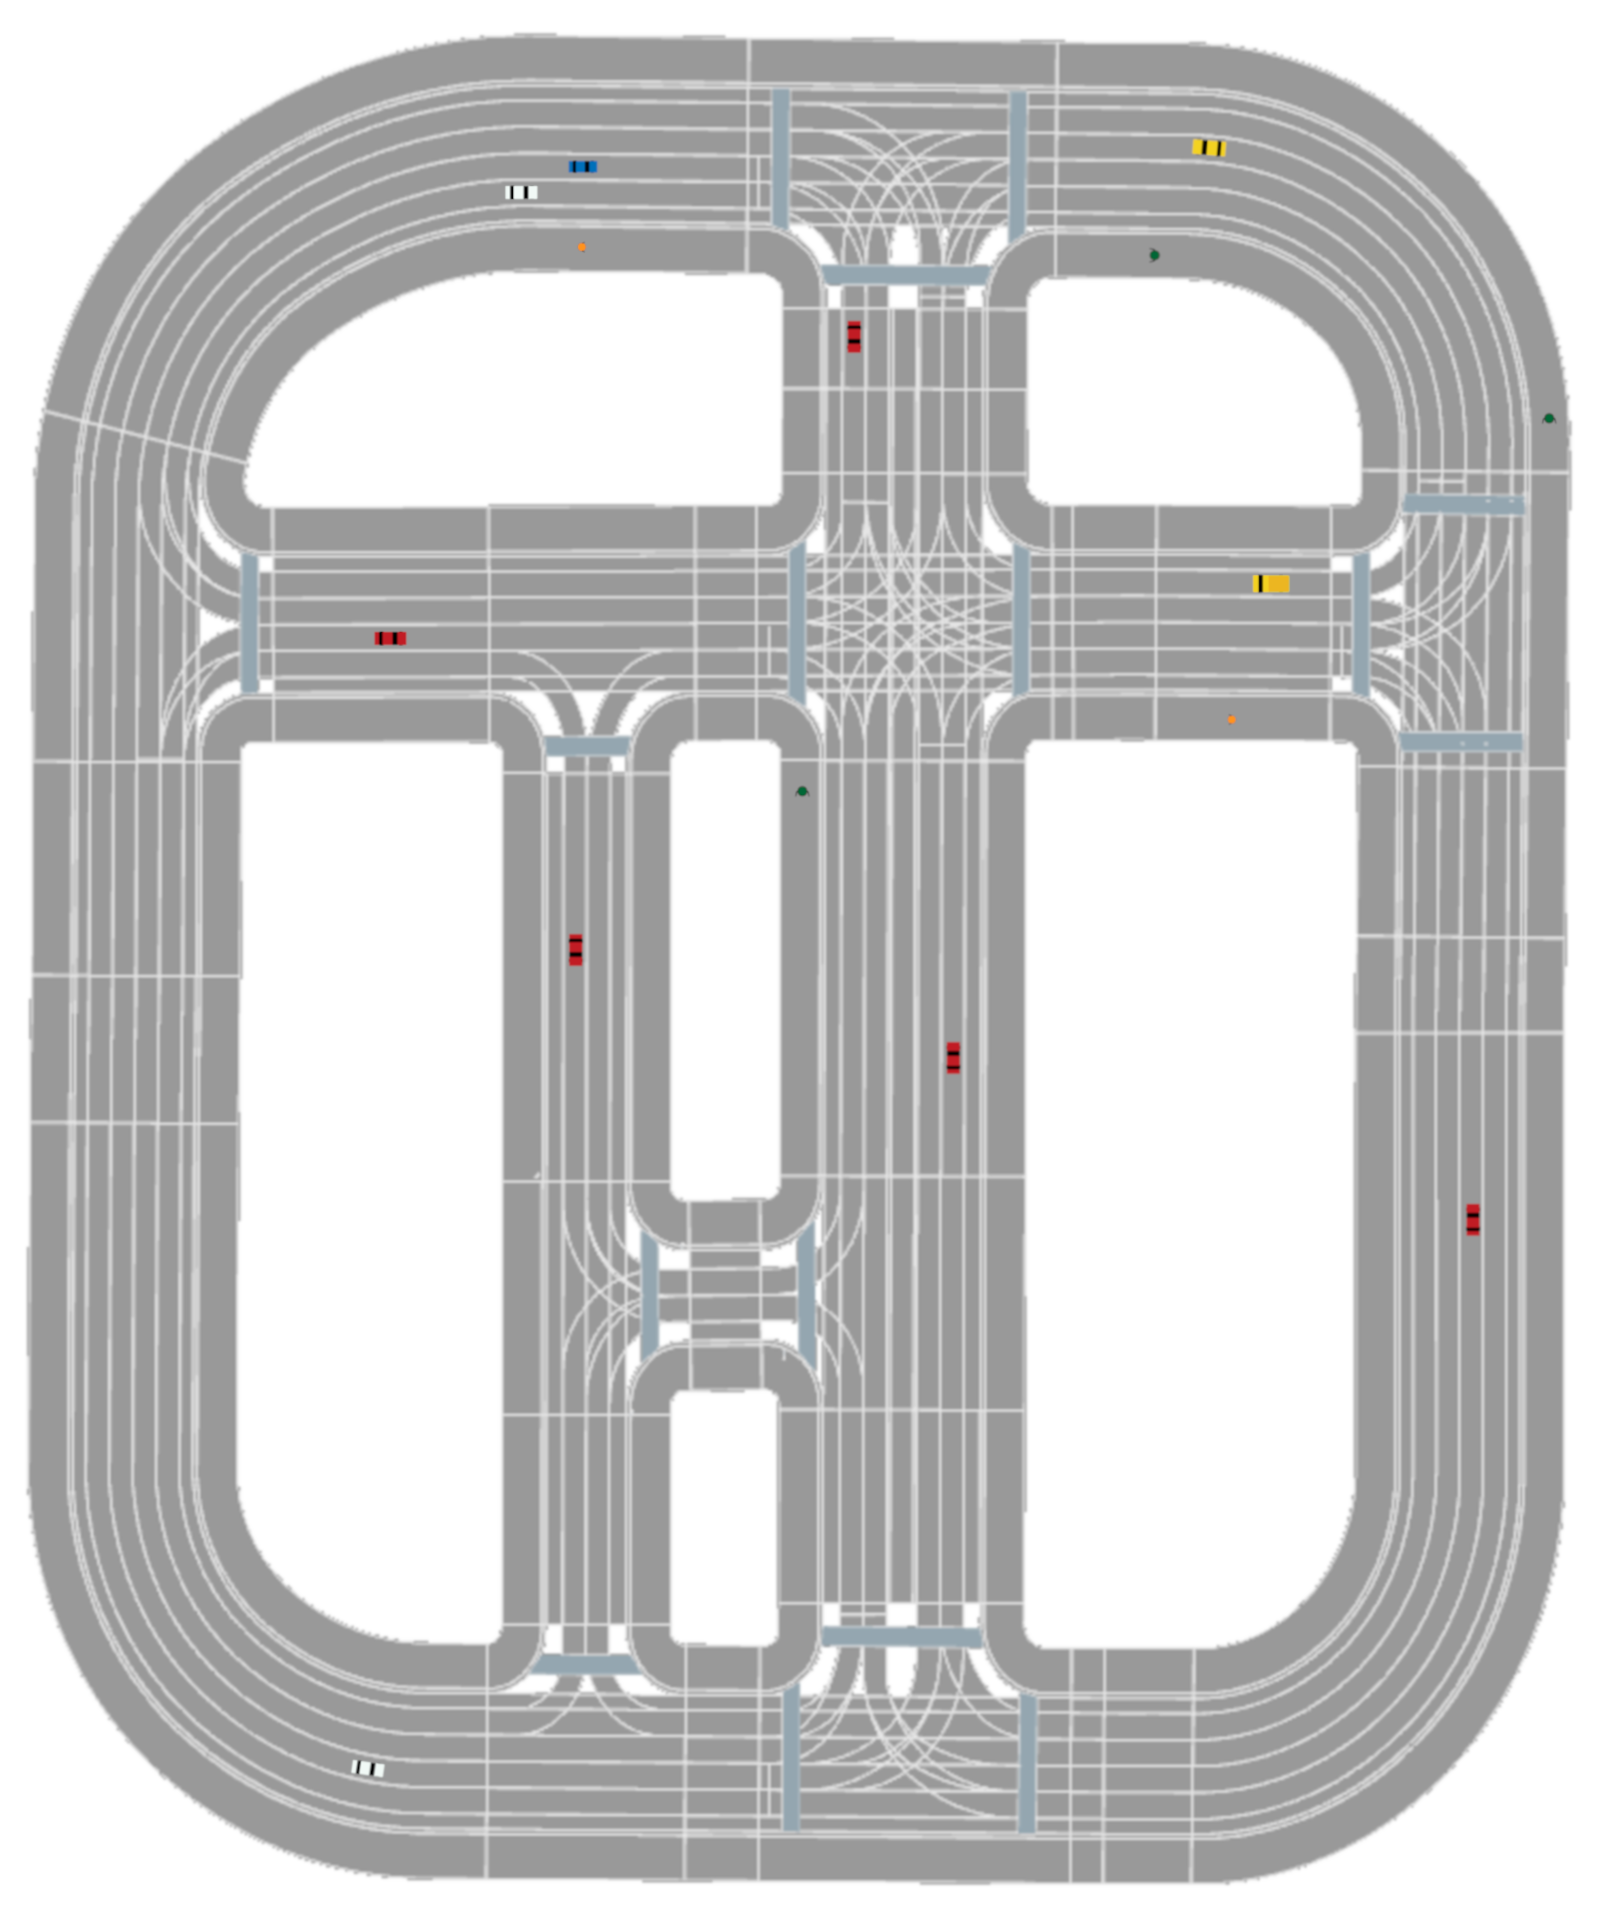
\includegraphics[width=1\linewidth]{figures/start_scenarios/scenario_2} 
		Start Scenario 2
	\end{minipage} 
	\caption{Visualization of Positions in Start Scenarios 1 and 2: Positions of all vehicles and pedestrians are depicted with the EGO vehicle drawn in blue.}
	\label{fig:appendix:start_scenarios_1_2} 
\end{figure}

\begin{figure}[ht] 
	\centering
	\begin{minipage}[b]{0.5\linewidth}
		\centering
		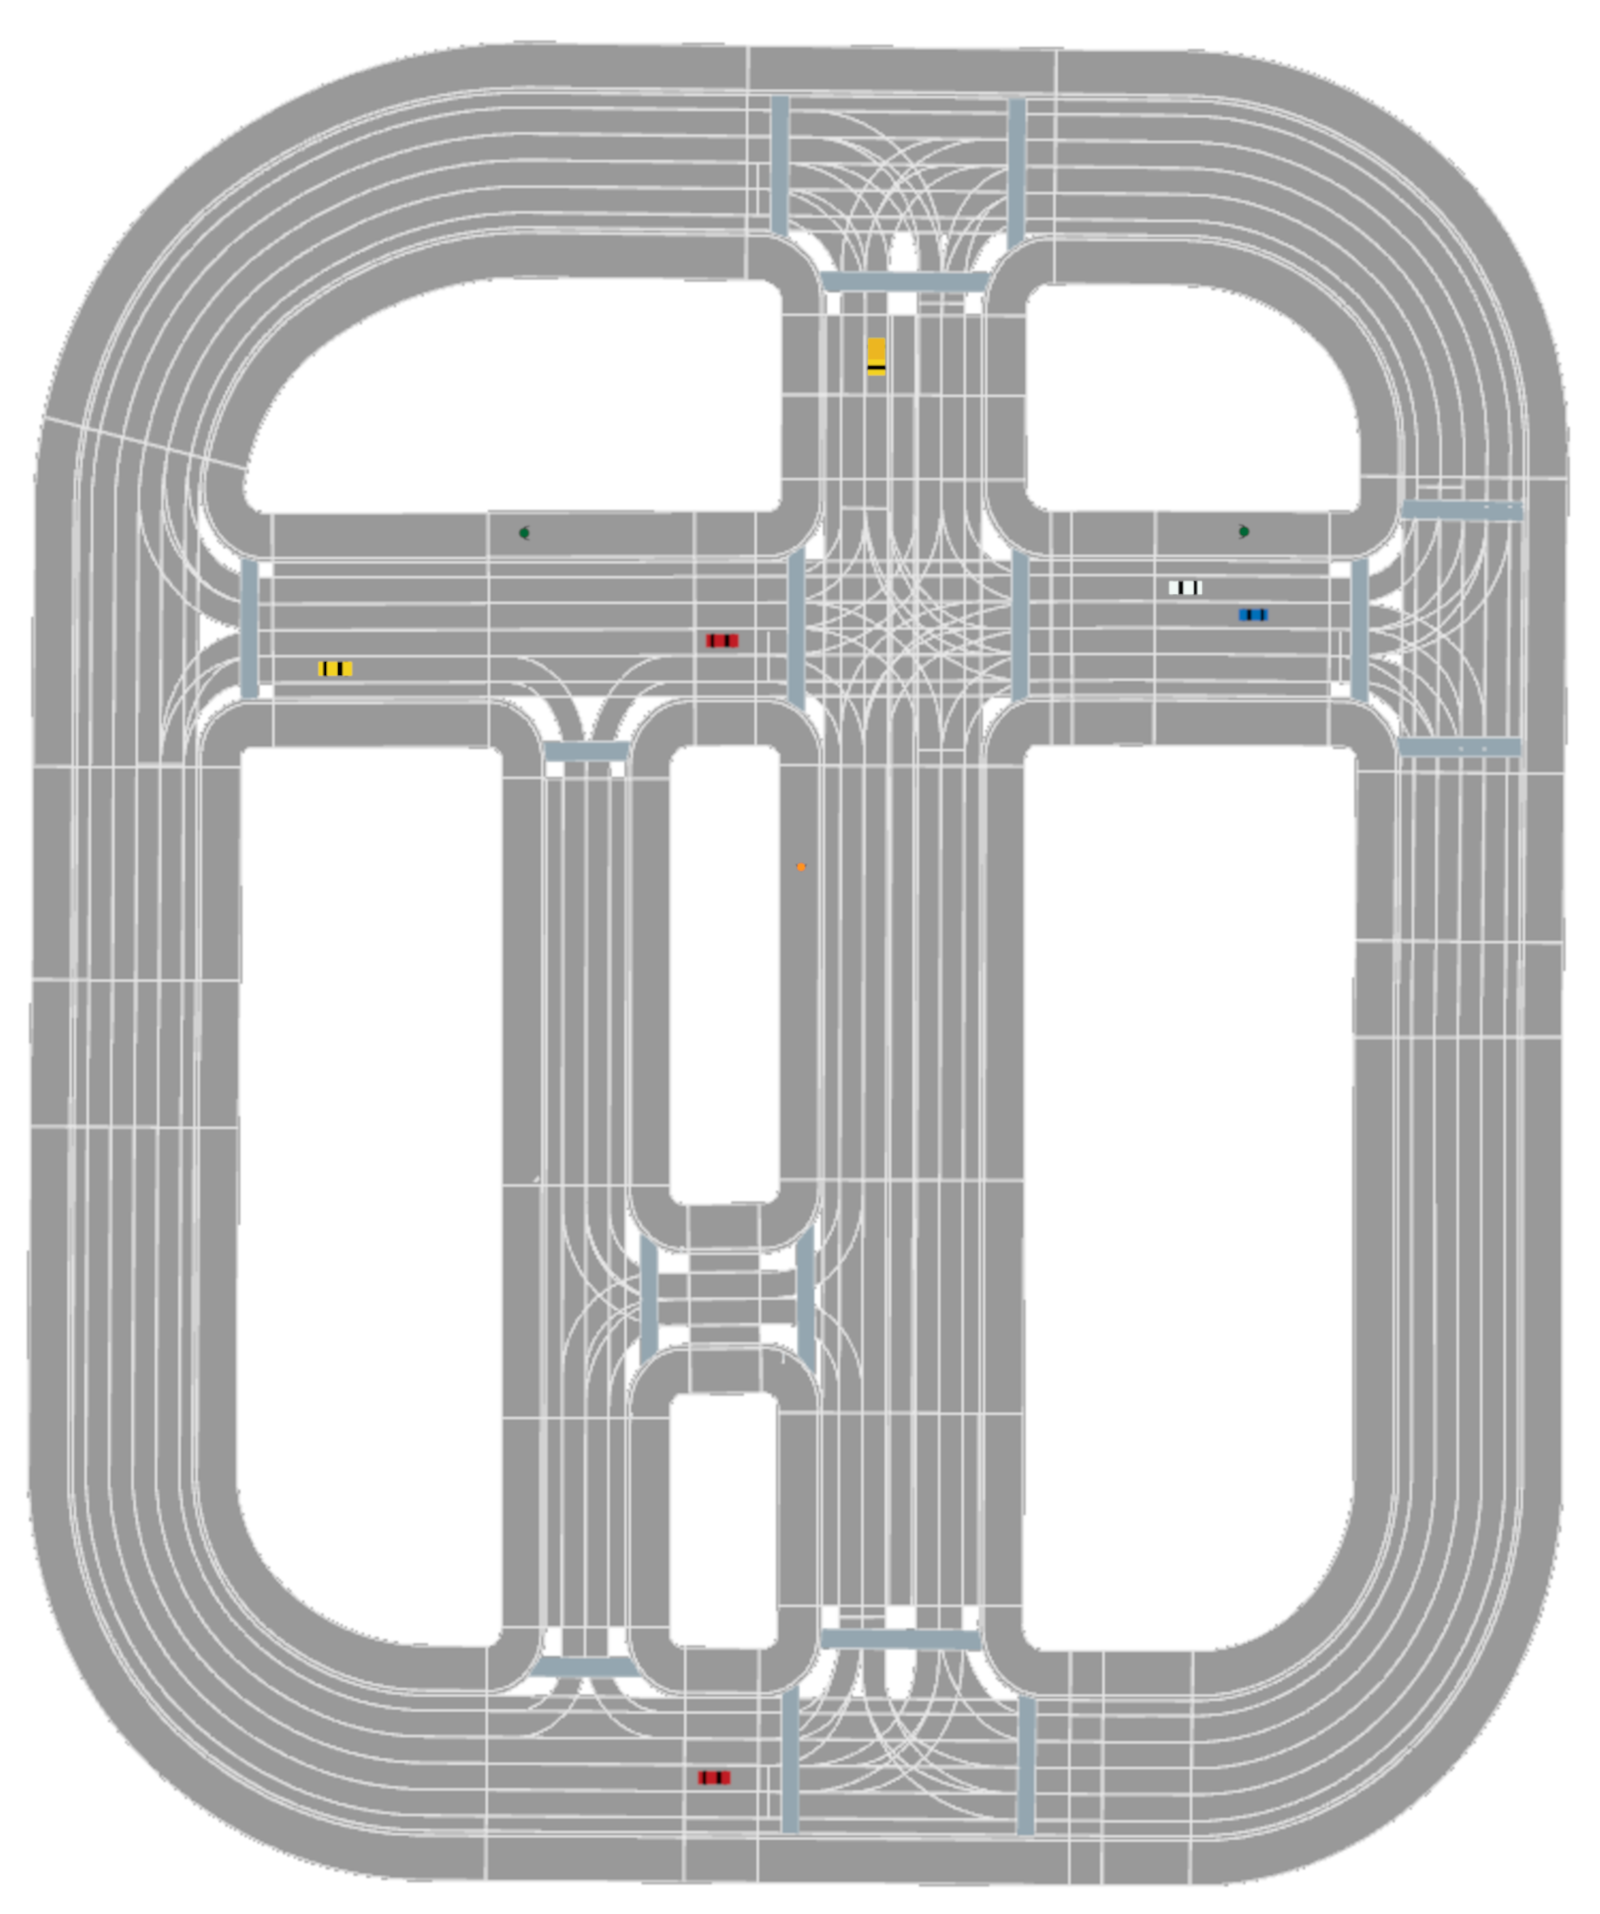
\includegraphics[width=1\linewidth]{figures/start_scenarios/scenario_3} 
		Start Scenario 3
	\end{minipage}%% 
	\begin{minipage}[b]{0.5\linewidth}
		\centering
		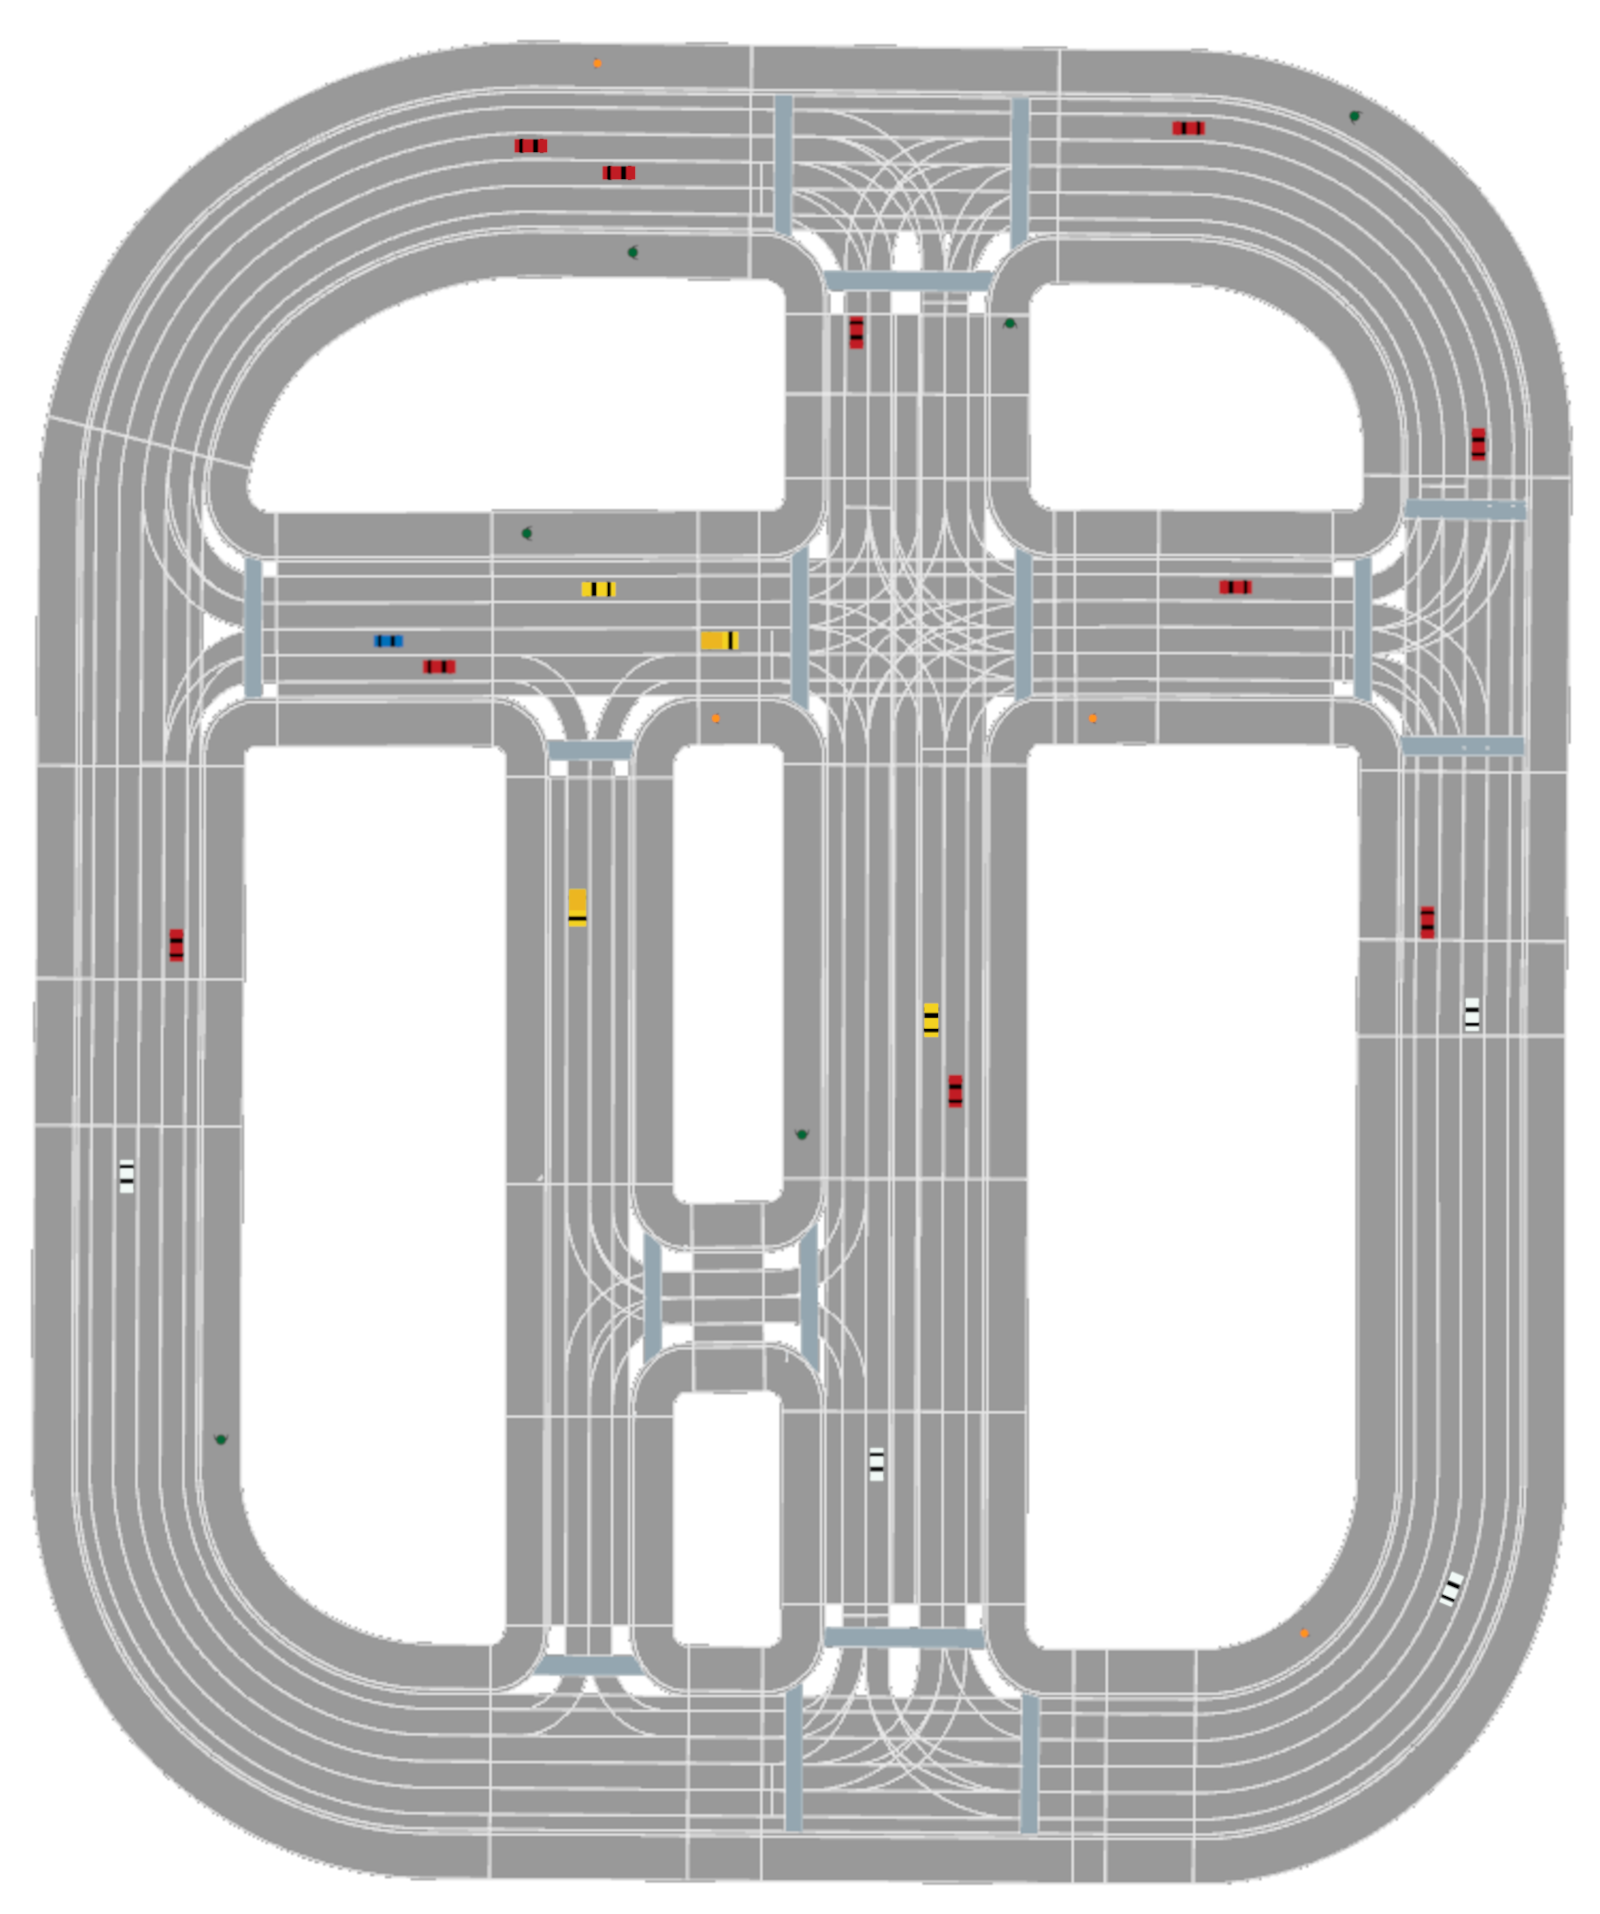
\includegraphics[width=1\linewidth]{figures/start_scenarios/scenario_4} 
		Start Scenario 4
	\end{minipage} 
	\caption{Visualization of Positions in Start Scenarios 3 and 4: Positions of all vehicles and pedestrians are depicted with the EGO vehicle drawn in blue.}
	\label{fig:appendix:start_scenarios_3_4} 
\end{figure}


\chapter{Appendix B.}

\begin{table}[ht]
	\centering
	\begin{tabular}{ rrrrrrrrr }
		\hline
		NO.& rep1 & rep2 & rep3 & rep4 & rep5 & rep6 & rep7 & rep8\\
  		\hline
		1 & 3.76 & 3.90 & 4.75 & 4.23 & 4.32 & 5.75 & 3.94 & 3.95 \\ 
		2 & 8.06 & 5.20 & 4.75 & 5.04 & 4.63 & 5.79 & 4.32 & 6.00 \\ 
		3 & 8.62 & 7.89 & 8.76 & 6.44 & 8.77 & 6.68 & 5.96 & 7.22 \\ 
		4 & 7.65 & 6.95 & 6.49 & 5.35 & 6.24 & 7.97 & 6.52 & 6.42 \\ 
		5 & 4.26 & 5.45 & 4.55 & 4.20 & 3.80 & 5.29 & 6.05 & 7.02 \\ 
		6 & 5.26 & 5.21 & 5.71 & 5.59 & 5.48 & 5.64 & 3.61 & 5.47 \\ 
		7 & 3.92 & 4.01 & 4.51 & 4.80 & 4.08 & 4.43 & 4.10 & 6.05 \\ 
		8 & 6.60 & 5.69 & 5.79 & 5.79 & 5.43 & 5.03 & 6.11 & 6.05 \\ 
		9 & 4.93 & 5.05 & 5.17 & 4.91 & 6.53 & 5.04 & 7.66 & 5.73 \\ 
		10 & 5.84 & 6.72 & 4.87 & 7.13 & 6.82 & 5.74 & 4.66 & 6.78 \\ 
		11 & 4.93 & 6.21 & 4.10 & 4.67 & 5.94 & 5.19 & 3.91 & 3.96 \\ 
		12 & 5.54 & 4.84 & 7.10 & 5.83 & 5.96 & 5.17 & 6.02 & 8.94 \\ 
		13 & 11.22 & 7.88 & 5.94 & 7.00 & 5.88 & 7.05 & 6.40 & 6.66 \\ 
		14 & 6.05 & 7.40 & 7.50 & 6.51 & 9.58 & 5.03 & 5.35 & 5.09 \\ 
		15 & 6.58 & 4.35 & 4.50 & 7.21 & 6.38 & 5.77 & 5.45 & 6.08 \\ 
		16 & 4.35 & 6.66 & 8.57 & 4.44 & 4.49 & 4.89 & 6.72 & 5.37 \\ 
		\hline
	\end{tabular}
	\caption{Table of Taguchi Experiment Results: A row corresponds to an experiment, each repeated eight times. The cumulated emergency break duration (in seconds) is shown.}
	\label{tab:appendix:hyperparameter_tuning_final_taguchi}
\end{table}

\begin{sidewaystable}
	\centering
	\begin{tabular}{ rrrrrrrrrrr }
		\hline
		scenario & rep1 & rep2 & rep3 & rep4 & rep5 & rep6 & rep7 & rep8 & rep9 & rep10\\
		\hline
		1 & 7.28 & 7.31 & 9.09 & 9.38 & 8.16 & 8.05 & 7.69 & 10.20 & 9.22 & 8.83 \\ 
		2 & 7.76 & 9.42 & 8.28 & 9.51 & 9.96 & 10.27 & 10.38 & 8.87 & 9.82 & 8.12 \\ 
		3 & 7.67 & 7.34 & 6.86 & 4.86 & 5.00 & 7.14 & 8.33 & 5.51 & 6.18 & 7.66 \\ 
		4 & 10.19 & 11.57 & 10.67 & 10.71 & 9.07 & 11.25 & 10.19 & 10.09 & 12.29 & 9.97 \\ 
		\hline
	\end{tabular}
	\caption{Optimized Genetic Algorithm Evaluation: The results of the optimized genetic algorithm over ten repetitions across four different start scenarios. The cumulated emergency break duration (in seconds) is shown.}
	\label{tab:appendix:evaluation_optimized}
	
	\vspace{2em}
	\begin{tabular}{ rrrrrrrrrrr }
		\hline
		scenario & rep1 & rep2 & rep3 & rep4 & rep5 & rep6 & rep7 & rep8 & rep9 & rep10\\
		\hline
		1 & 6.66 & 6.10 & 6.32 & 7.32 & 7.37 & 9.23 & 6.44 & 8.57 & 6.14 & 6.70 \\
		2 & 7.09 & 6.78 & 7.00 & 7.10 & 6.01 & 8.04 & 6.75 & 8.59 & 9.13 & 8.12 \\ 
		3 & 8.31 & 6.14 & 6.94 & 8.99 & 5.27 & 4.94 & 6.56 & 6.03 & 6.61 & 5.11 \\ 
		4 & 8.78 & 9.44 & 8.22 & 7.47 & 7.99 & 9.58 & 9.45 & 8.59 & 6.90 & 8.17 \\ 
		\hline
	\end{tabular}
	\caption{Default Genetic Algorithm Evaluation: The results of the default genetic algorithm over ten repetitions across four different start scenarios. The cumulated emergency break duration (in seconds) is shown.}
	\label{tab:appendix:evaluation_default}
	
	\vspace{2em}
	\begin{tabular}{ rrrrrrrrrrr }
		\hline
		scenario & rep1 & rep2 & rep3 & rep4 & rep5 & rep6 & rep7 & rep8 & rep9 & rep10\\
		\hline
		1 & 3.92 & 4.41 & 4.19 & 4.33 & 4.38 & 4.88 & 8.27 & 4.76 & 5.65 & 4.64 \\ 
		2 & 5.16 & 4.91 & 4.82 & 4.89 & 4.91 & 5.47 & 4.97 & 6.21 & 4.93 & 4.99 \\ 
		3 & 4.53 & 4.63 & 4.35 & 4.62 & 4.13 & 4.14 & 4.91 & 5.98 & 4.56 & 4.34 \\ 
		4 & 7.01 & 6.01 & 6.63 & 7.31 & 6.85 & 6.66 & 7.35 & 6.78 & 7.38 & 6.57 \\
		\hline
	\end{tabular}
	\caption{Random Search Evaluation: The results of the random search over ten repetitions across four different start scenarios. The cumulated emergency break duration (in seconds) is shown.}
	\label{tab:appendix:evaluation_random}
\end{sidewaystable}





